
%%%%%%%%%%%%%%%%%%%%%%%%%%%%%%%%%%%%%%%%%%%%%%%%%%%%%%%%%
%%% {{.Q.Title}}
%%%%%%%%%%%%%%%%%%%%%%%%%%%%%%%%%%%%%%%%%%%%%%%%%%%%%%%%%

\begin{frame}[plain]{ {{.Q.Title}} }
\begin{columns}[onlytextwidth]
\begin{column}{0.75\textwidth}
偏心受压柱,已知:\\
柱计算高度:$l_c= {{.Q.L_c}} m$ 。 \\
矩形截面:$b \times h = {{.Q.B}} \times {{.Q.H}} mm^2$。\\
材料:采用纵筋~{{.Q.S}},{{.Q.C}} 混凝土。\\
内力:$(M_t, M_b, N) = ( {{.Q.M_t}} kN\cdot m, {{.Q.M_b}} kN\cdot m, {{.Q.N}} kN)$ \\
按对称配筋柱计算所需纵筋(取$a_s = {{.Q.D_s}} mm, a'_s = {{.Q.D_ss}} mm$)。\\
\end{column}

\begin{column}{0.25\textwidth}
\begin{center}
\scalebox{0.5}{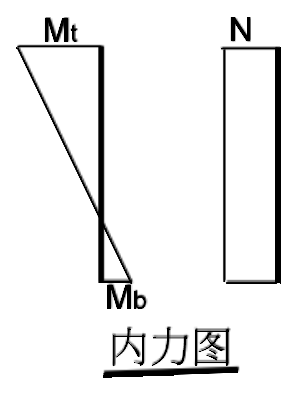
\includegraphics{fig1.eps}}
\end{center}
\end{column}

\end{columns}
\end{frame}

\begin{frame}[plain]
解:一、二阶效应的计算
\vspace{-0.5em}
\begin{align*}
	& h_0 = h - a_s = {{.Q.H}} - {{.Q.D_s}} = {{.H_0}} mm &\\ 
	\uncover<2-> {& M_2 = max(|M_t|, |M_b|)= {{.M_2}} kN\cdot m &\\ 
	& M_1 = \frac{M_t\cdot M_b}{|M_t|\cdot|M_b|}min(|M_t|, |M_b|)= {{.M_1}} kN\cdot m  &\\}
	\uncover<3-> {& \frac{M_1} {M_2} = \frac{ {{.M_1}} } { {{.M_2}} } = {{printf "%5.3f" .M_1DividedByM_2}} } &\\
	\uncover<4-> {& i = h/\sqrt{12} = {{.Q.H}} / \sqrt{12} = {{printf "%5.1f" .I}} mm  &\\}
	\uncover<5-> {& \frac{l_c} {i} = \frac{ {{.Q.L_c}}\times10^3 } { {{printf "%5.1f" .I}} } =  {{printf "%6.1f" .Lambda}} &\\ }
	\uncover<6-> {& \frac{N}{f_cA} = \frac{ {{.Q.N}}\times10^3 }{ {{.Fc}}\times {{.Q.B}}\times {{.Q.H}} } = {{printf "%6.3f" .NDividedByFcA}}&}
\end{align*}
\end{frame}

%%% M_1/M_2 > 0.9
%%%{{if .M_1DividedByM_2GreatThanDotNine}}
%%%
\begin{frame}[plain]
\vspace{-0.5em}
\begin{align*}
	\uncover<2-> {& \text{因为}\frac{M_1}{M_2}= {{printf "%5.3f" .M_1DividedByM_2}} < 0.9 &\\}
\end{align*}
\uncover<3-> {所以:要考虑附加弯矩\\}
\vspace{-1.5em}
\begin{align*}
	\uncover<4-> {&C_m = max(0.7, 0.7+0.3M_1/M_2) &\\ 
	\mspace{9mu} &= max(0.7, 0.7+0.3\times{{.M_1}} / {{.M_2}} )={{printf "%5.3f" .Cm}} &\\}
	\uncover<5->{& e_a = max(20, {{.Q.H}}/30) = {{printf "%3.0f" .E_a}}mm  &\\ }
	\uncover<6->{& \zeta_c = min(1.0, \frac{0.5f_cA}{N}) 
			= min(1.0, 0.5\times {{printf "%5.3f" .NDividedByFcA}})={{printf "%5.3f" .Zeta_c}} &\\ }
\end{align*}
\end{frame}

%%%%%%%
\begin{frame}[plain]
\vspace{-0.5em}
\begin{align*}
	\uncover<2->{& \eta_{ns} = 1+ \frac{1}{1300(M_2/N + e_a)/h_0}(\frac{l_c}{h})^2 \zeta_c &\\}
	\uncover<3->{& \mspace{9mu} = 1+\frac{ {{.H_0}} }{1300( {{.M_2}}/{{.Q.N}}\times 10^3+ {{printf "%4.0f" .E_a}})}
						(\frac{ {{.Q.L_c}}\times10^3 }{ {{.Q.H}} } )^2\times {{printf "%5.3f" .Zeta_c}} &\\
		     &= {{printf "%5.3f" .Eta_ns}} &\\}
	\uncover<4->{& M = max(1.0, C_m \eta_{ns}) &\\
		     & \mspace{10mu}= max(1.0, {{printf "%5.3f" .Cm}}\times {{printf "%5.3f" .Eta_ns}})\times {{.M_2}} &\\
		     &= {{printf "%6.1f" .M}} &\\}
\end{align*}
\end{frame}

%%% N/(f_c A) > 0.9
%%%{{else if .NDividedByFcAGreatThanDotNine}}
%%%
\begin{frame}[plain]
\vspace{-0.5em}
\begin{align*}
	\uncover<2-> {&\text{因为}  \frac{N}{f_c A} = {{printf "%6.3f" .NDividedByFcA}} > 0.9 &\\}
\end{align*}
\uncover<3-> {所以:要考虑附加弯矩\\}
\vspace{-1.5em}
\begin{align*}
	\uncover<4-> {&C_m = max(0.7, 0.7+0.3M_1/M_2) &\\ 
	\mspace{9mu} &= max(0.7, 0.7+0.3\times{{.M_1}} / {{.M_2}} )={{printf "%5.3f" .Cm}} &\\}
	\uncover<5->{& e_a = max(20, {{.Q.H}}/30) = {{printf "%3.0f" .E_a}}mm  &\\ }
	\uncover<6->{& \zeta_c = min(1.0, \frac{0.5f_cA}{N}) 
			= min(1.0, 0.5\times {{printf "%5.3f" .NDividedByFcA}})={{printf "%5.3f" .Zeta_c}} &\\ }
\end{align*}
\end{frame}

%%%%%%%
\begin{frame}[plain]
\vspace{-0.5em}
\begin{align*}
	\uncover<2->{& \eta_{ns} = 1+ \frac{1}{1300(M_2/N + e_a)/h_0}(\frac{l_c}{h})^2 \zeta_c &\\}
	\uncover<3->{& \mspace{9mu} = 1+\frac{ {{.H_0}} }{1300( {{.M_2}}/{{.Q.N}}\times 10^3+ {{printf "%4.0f" .E_a}})}
						(\frac{ {{.Q.L_c}}\times10^3 }{ {{.Q.H}} } )^2\times {{printf "%5.3f" .Zeta_c}} &\\
		     &= {{printf "%5.3f" .Eta_ns}} &\\}
	\uncover<4->{& M = max(1.0, C_m \eta_{ns}) &\\
		     & \mspace{10mu}= max(1.0, {{printf "%5.3f" .Cm}}\times {{printf "%5.3f" .Eta_ns}})\times {{.M_2}} &\\
		     &= {{printf "%6.1f" .M}} &\\}
\end{align*}
\end{frame}
%%%
%%%{{else if .LambdaGreatThanLambdaLimit}}
%%%
\begin{frame}[plain]
因为
\begin{align*}
	\uncover<2-> {&
	\frac{l_c} {i} = {{printf "%6.1f" .Lambda}} >  34 - 12(M_1/M_2) = 34 - 12 \times {{printf "%6.1f" .M_1DividedByM_2}} 
	= {{printf "%6.1f" .LambdaLimit}} &} 
\end{align*}
\uncover<3-> {所以:要考虑附加弯矩\\}
\vspace{-1.5em}
\begin{align*}
	\uncover<4-> {&C_m = max(0.7, 0.7+0.3M_1/M_2) &\\ 
	\mspace{9mu} &= max(0.7, 0.7+0.3\times{{.M_1}} / {{.M_2}} )={{printf "%5.3f" .Cm}} &\\}
	\uncover<5->{& e_a = max(20, {{.Q.H}}/30) = {{printf "%3.0f" .E_a}}mm  &\\ }
	\uncover<6->{& \zeta_c = min(1.0, \frac{0.5f_cA}{N}) = min(1.0, 0.5\times {{printf "%5.3f" .NDividedByFcA}})={{printf "%5.3f" .Zeta_c}} &\\ }
\end{align*}
\end{frame}

\begin{frame}[plain]
\vspace{-0.5em}
\begin{align*}
	\uncover<2->{& \eta_{ns} = 1+ \frac{1}{1300(M_2/N + e_a)/h_0}(\frac{l_c}{h})^2 \zeta_c &\\}
	\uncover<3->{& \mspace{9mu} = 1+\frac{ {{.H_0}} }{1300( {{.M_2}}/{{.Q.N}}\times 10^3+ {{printf "%4.0f" .E_a}})}
					(\frac{ {{.Q.L_c}}\times10^3 }{ {{.Q.H}} } )^2\times {{printf "%5.3f" .Zeta_c}} &\\
	&= {{printf "%5.3f" .Eta_ns}} &\\}
	\uncover<4->{& M = max(1.0, C_m \eta_{ns}) &\\
		     & \mspace{10mu}= max(1.0, {{printf "%5.3f" .Cm}}\times {{printf "%5.3f" .Eta_ns}})\times {{.M_2}} &\\
		&= {{printf "%6.1f" .M}} &\\}
\end{align*}
\end{frame}

%%%
%%%{{else}}
%%%
\begin{frame}[plain]
\vspace{-0.5em}
因为
\begin{align*}
	\uncover<2-> {(1)\quad & \frac{l_c} {i} = {{printf "%6.1f" .Lambda}} <  &\\ 
			&34 - 12(M_1/M_2) = 34 - 12 \times {{printf "%6.1f" .M_1DividedByM_2}} = {{printf "%6.1f" .LambdaLimit}} &\\} 
	\uncover<3-> {(2)\quad & \frac{M_1}{M_2}= {{printf "%5.3f" .M_1DividedByM_2}} < 0.9 &\\}
	\uncover<4-> {(3)\quad & \frac{N}{f_c A} = {{printf "%6.3f" .NDividedByFcA}} < 0.9 &\\}
\end{align*} 
\uncover<5-> {所以:不用考虑二阶效应,取 $M = M_2 = {{.M_2}}kN\cdot m $}
\end{frame}
%%%{{end}}

\begin{frame}[plain]
二、偏心距的计算 
\beamerdefaultoverlayspecification{<+-}
\begin{align*}
	& e_0 = \frac{M} {N} = \frac{ {{.M}} } { {{.Q.N}}} m = {{printf "%3.0f" .E_0}} mm &\\
	\uncover<2->{& e_a = max(20, {{.Q.H}}/30) = {{printf "%3.0f" .E_a}}mm  &\\ }
	\uncover<3->{& e_i = e_0 + e_a = {{printf "%3.0f" .E_0}} + {{printf "%3.0f" .E_a}} = {{printf "%4.0f" .E_i}} mm &\\ }  
	\uncover<4->{& e = e_i + 0.5h - a_s &\\ 
		     &\mspace{9mu} = {{printf "%4.0f" .E_i}} + 0.5 \times {{.Q.H}} - {{.Q.D_s}} = {{printf "%6.0f" .E}} mm &\\}  
	\uncover<5->{& e' = e_i - 0.5h + a'_s &\\ 
		     &\mspace{9mu} = {{printf "%4.0f" .E_i}} - 0.5 \times {{.Q.H}} + {{.Q.D_s}} = {{printf "%6.0f" .Ee}} mm &\\}  
\end{align*} 
\end{frame}

\begin{frame}[plain]
三、假设为受拉破坏
\begin{align*}
	& x = \frac{N} {\alpha_1 f_c b} = \frac{ {{.Q.N}}\times 10^3} {1.0 \times {{.Fc}} \times {{.Q.B}} } = {{printf "%6.1f" .X}} mm &
\end{align*}
%%%{{if .XiGreatThanXi_b}}
%%% 受拉纵筋不屈服
\begin{align*}
	\uncover<2->{ &x > \xi_b h_0 = {{.Xi_b}}\times{{.H_0}}={{printf "%5.1f" .X_b}}, \text{假设错误,按受压破坏计算} &\\}
	\uncover<3->{ &\xi = \frac{%%frac first part
				N-\xi_b\alpha_1 f_c bh_0}{\frac{Ne - 0.43\alpha_1 f_c bh^2_0
			}{%%frac second part
				(\beta_1 - \xi_b)(h_0 - a'_s)
			}%%end frac
			+ \alpha_1 f_c bh_0} + \xi_b &\\ 
		      &\mspace{10mu}= \frac{%%frac first
				{{.Q.N}}\times10^3 - {{.Xi_b}}\times1.0\times{{.Fc}}\times{{.Q.B}}\times{{.H_0}}~
			}{%%frac second
				\frac{%%%frac first
					{{.Q.N}}\times10^3\times{{.E}}-0.43\times1.0\times{{.Fc}}\times{{.Q.B}}\times{{.H_0}}^2~
				}{%%%frac second
					(0.8-{{.Xi_b}})({{.H_0}}-{{.Q.D_ss}})~
				}
				+ 1.0\times{{.Fc}}\times{{.Q.B}}\times{{.H_0}}~
			} &\\
			 &\mspace{14mu}+  {{.Xi_b}} = {{printf "%6.3f" .Xi}} &\\
		}
	\uncover<4->{&A_s=A'_s = \frac{%%frac first
				Ne - \alpha_1 f_c bh^2_0 \xi(1-0.5\xi)
			}{%%frac seconcd
				f'_y(h_0 - a'_s)	
			} &\\
		  &\mspace{10mu}\frac{%%frac first
				{{.Q.N}}(10^3)\times {{.E}} - 1.0\times{{.Fc}}\times{{.Q.B}}\times{{.H_0}}^2\times{{printf "%5.3f" .Xi}}(1-0.5\times{{printf "%5.3f" .Xi}})
			}{%%frac seconc
				{{.Fyy}}\times({{.H_0}} - {{.Q.D_ss}})
			} &\\
		   &\mspace{10mu} = {{printf "%7.1f" .As}} mm^2 \text{配筋率验算略}	&
		}		
\end{align*}
%%%
%%%{{else if .XLessThanDoubleD_ss}}
%%% 受压纵筋不屈服
\begin{align*}
	\uncover<2-> { & < 2a'_s = 2\times {{.Q.D_ss}} = {{printf "%4.1f" .DoubleD_ss}} mm &\\ }
	\uncover<3-> { & \text{假设正确,但受压纵筋不屈服。} &\\ 
		& A_s = A'_s = \frac{Ne'}{f\mspace{3mu}'_y(h_0 - a'_s)}\mspace{10mu} &\\ 
	       	& = \frac{ {{.Q.N}} \times 10^3 \times {{printf "%6.0f" .Ee}} }{ {{.Fyy}}\times ({{.H_0}} - {{printf "%4.1f" .Q.D_ss}} )} &\\
	       	&\mspace{10mu} = {{printf "%6.1f" .As}} }
\end{align*}
%%%%
%%%{{else}} 
\begin{align*}
	\uncover<2-> { & > 2a'_s = 2\times {{.Q.D_ss}} = {{printf "%4.1f" .DoubleD_ss}} mm &\\ 
		       & < \xi_b \times h_0 = {{.Xi_b}} \times {{.H_0}} = {{printf "%6.1f" .X_b}} mm &\\ } 
	\uncover<3-> { & \text{假设正确,且受压纵筋能屈服。} &\\ 
	     	& A_s = A'_s = \frac{Ne - \alpha_1 f_c b x (h_0 - 0.5x)}{f\mspace{3mu}'_y(h_0 - a'_s)} \mspace{10mu}&\\ 
		& = \frac{ {{.Q.N}} \times 10^3 \times {{printf "%6.0f" .E}} - 1.0 \times {{.Fc}} \times {{.Q.B}} 
		\times {{printf "%6.1f" .X}} \times ({{.H_0}} - 0.5 \times {{printf "%6.1f" .X}} )} 
		{ {{.Fyy}} \times ({{.H_0}} - {{printf "%4.1f" .Q.D_ss}}) } &\\
	    	& \mspace{10mu} = {{printf "%6.1f" .As}} mm^2 &\\ }
\end{align*}
%%%{{end}}
%%%
%%% 配筋率验算
\begin{align*} 
%%%{{if .AsGreatThanAs_min}}	
	\uncover<4-> { & > 0.2\% \times {{.Q.B}} \times {{.Q.H}} = {{printf "%6.1f" .As_min}} mm^2 \text{,单侧配筋率满足要求}&\\ }
%%%{{else}} 
	\uncover<4-> { & < 0.2\% \times {{.Q.B}} \times {{.Q.H}} = {{printf "%6.1f" .As_min}} mm^2 \text{,配筋时按}As_min\text{取值}&\\ }
%%%{{end}}
%%%
%%%{{if .AsPlusAssGreatThanAsPlusAss_min}}
	\uncover<5-> { & A_s+A'_s > {{.TwoSidesRho_min}}\% \times {{.Q.B}} \times {{.Q.H}} 
	= {{printf "%6.1f" .AsPlusAss_min}} mm^2 \text{,双侧配筋率满足要求}&\\ }
%%%{{else}}
	\uncover<5-> { & A_s+A'_s < {{.TwoSidesRho_min}}\% \times {{.Q.B}} \times {{.Q.H}} 
	= {{printf "%6.1f" .AsPlusAss_min}} mm^2 \text{,配筋时应满足全配筋率要求}&\\ }
%%%{{end}}
\end{align*}
\end{frame}


